\documentclass[11pt]{article}
\usepackage[margin = 1in]{geometry}
\usepackage{amsmath}
\usepackage{amssymb}
\usepackage{amsthm}
\usepackage{graphicx}
\usepackage{subfig}
\usepackage{enumitem}
\usepackage{url}
\usepackage[parfill]{parskip}
\newcommand{\skipline}{\vspace{\baselineskip}}
\newenvironment{problem}[1]{\textbf{Problem #1: }}{\newpage}


\begin{document}
	
	\begin{center}
		\textbf{Homework 1} \\
		\textbf{Ordinary Differential Equations} \\
		\textbf{Math 537} \\
		\textbf{Stephen Giang} \\
	\end{center}
	\skipline
	Solve the following problems, discuss results, and perform linear stability analysis near equilibrium points.
	\\ \\
	\begin{problem}{1}
		$$\frac{dx}{dt} = f(x),$$
		here (i) $f(x) = x$; (ii) $f(x) = x^2$; and (iii) $f(x) = x^3$
		\\	
		\begin{enumerate}[label = (\alph*)]
			\item Perform (linear) stability analysis.
			\begin{enumerate}[label = (\roman*)]
				\item For $x' = f(x) = x$, we get the fixed point $x_c = 0$.  We can now see that because $f'(0) = 1 > 0$, the critical point is unstable. \\  
				We can see that for $x < 0$, we get $x' < 0$, and for $x > 0$, we get $x'> 0$, thus giving us a source. 
				\begin{figure}[h!]
					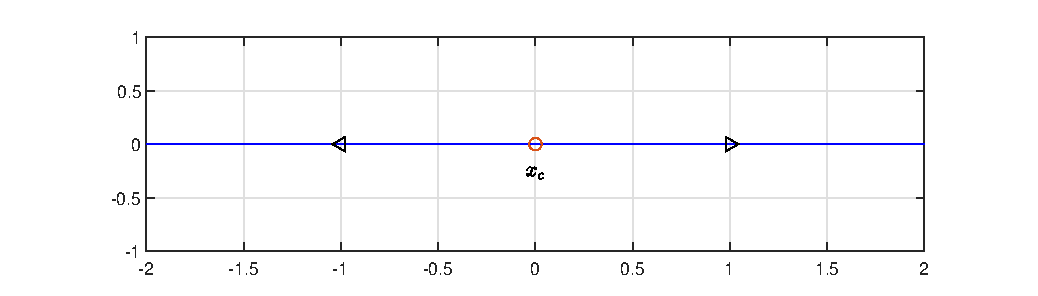
\includegraphics[width = 16cm, height = 5cm]{PhaseLine1i.eps}
				\end{figure}
				\item For $x' = f(x) = x^2$, we get the fixed point $x_c = 0$.  We notice that because $f'(0) = 0$, the critical point is half-stable.  \\
				We can see that for $x < 0$, we get $x' > 0$, and for $x > 0$, we get $x'> 0$, thus giving us a saddle point.
				\begin{figure}[h!]
					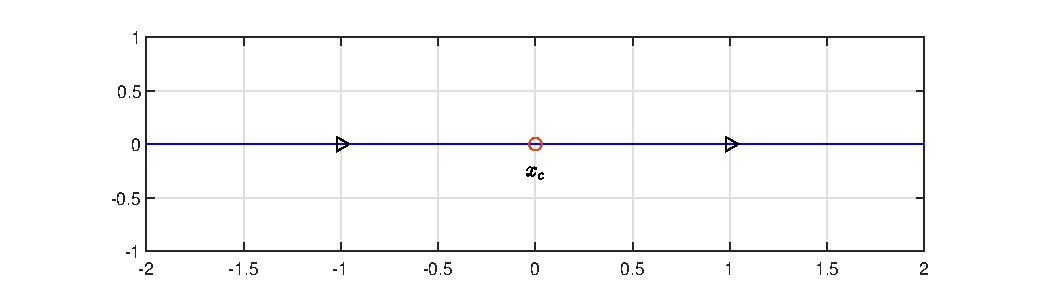
\includegraphics[width = 16cm, height = 5cm]{PhaseLine1ii.eps}
				\end{figure}
				\newpage
				\item For $x' = f(x) = x^3$, we get the fixed point $x_c = 0$.  We notice that because $f'(0) = 0$, the critical point is half-stable.  \\ 
				We can see that for $x < 0$, we get $x' < 0$, and for $x > 0$, we get $x'> 0$, thus giving us a source.
				\begin{figure}[h!]
					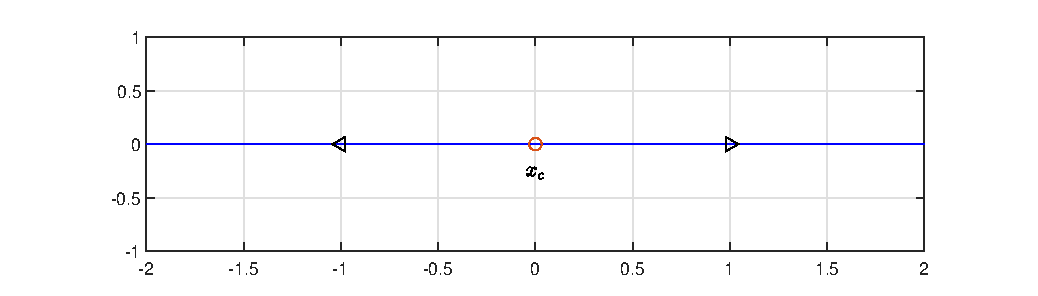
\includegraphics[width = 16cm, height = 5cm]{PhaseLine1i.eps}
				\end{figure}
			\end{enumerate} 
			\newpage
			\item Find and analyze the corresponding solutions
			\begin{enumerate}[label = (\roman*)]
				\item $\frac{dx}{dt} = f(x) = x$: (Separable)
				\begin{align*}
					\frac{dx}{dt} &= x & \ln x &= t + C \\
					\int \frac{dx}{x} &= \int dt & x &= Ce^{t}
				\end{align*}
				If we let $x(0) = x_0$, we get the following solution:
				$$x = x_0e^t $$
				Now we can see that as $t \rightarrow -\infty$, $x \rightarrow 0$, and as $t \rightarrow \infty$, $x \rightarrow \infty$. \\
				\item $\frac{dx}{dt} = f(x) = x^2$: (Separable)
				\begin{align*}
					\frac{dx}{dt} &= x^2 & \frac{-1}{x} &= t + C \\
					\int \frac{dx}{x^2} &= dt & x &= \frac{-1}{t + C}
				\end{align*}
				If we let $x(0) = x_0$, we get the following solution:
				$$x = \frac{x_0}{-x_0\,t + 1} $$
				Now we can see that as $t \rightarrow -\infty$, $x \rightarrow 0$, and as $t \rightarrow \infty$, $x \rightarrow 0$. \\
				\item $\frac{dx}{dt} = f(x) = x^3$: (Separable)
				\begin{align*}
					\frac{dx}{dt} &= x^3 & \frac{1}{-2x^2} &= t + C \\
					\int \frac{dx}{x^3} &= dt & x &= \pm\sqrt{\frac{1}{-2t + C} }
				\end{align*}
				If we let $x(0) = x_0$, we get the following solution:
				$$x = \pm\sqrt{\frac{x_0^2}{-2tx_0^2 + 1} }$$
				Now we can see that as $t \rightarrow -\infty$, $x \rightarrow 0$. Because we cannot have a negative inside the radical, we get undefined values of $x$, as $t \rightarrow \infty$.
			\end{enumerate}
		\end{enumerate}
	\end{problem}
	
	\begin{problem}{2}
		$$\frac{dx}{dt} = x^2 - 2x$$
		\\
		Notice we can find fixed points, when $f(x) = x^2 - 2x = 0$.  We can see that we get the following fixed points: $x_c = 0, 2$.
		\\ \\ 
		We can now see that because $f'(0) = -2 < 0$, the critical point is stable. 
		\\ 
		We can see that for $x < 0$, we get $x' > 0$, and for $0 < x < 2$, we get $x' <  0$, thus giving us a sink.
		\\ \\
		We can now see that because $f'(2) = 2 > 0$, the critical point is unstable. 
		\\ 
		We can see that for $0 < x < 2$, we get $x' < 0$, and for $x > 2$, we get $x' >  0$, thus giving us a source.
		\\ \\
		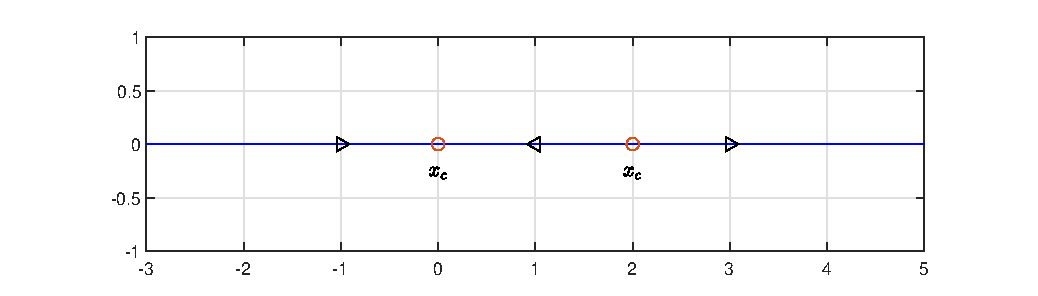
\includegraphics[width = 16cm, height = 5cm]{PhaseLine2.eps}
		\\ \\
		Notice the solution for $\frac{dx}{dt} = x^2 - 2x$: (Bernoulli's with $\mu = \frac{1}{x}$ and $\frac{d\mu}{dt} = \frac{-1}{x^2}\frac{dx}{dt}$)
			\begin{align*}
				\frac{dx}{dt} + 2x &= x^2 & \int \frac{d\mu}{2\mu - 1} &= \int dt\\
				\frac{d\mu}{dt} - 2\mu &= - 1 & \mu &= \frac{Ce^{2t} + 1}{2}
			\end{align*}
		Thus we get the following solution after resubstitution after solving for C with $x(0) = x_0$:
			$$x = \frac{2x_0}{(2 - x_0)e^{2t} + x_0} $$
		Now we can see that as $t \rightarrow -\infty$, $x \rightarrow 2$, and as $t \rightarrow \infty$, $x \rightarrow 0$. 
	\end{problem}
	
	\begin{problem}{3}
		$$\frac{dx}{dt} = -(\alpha x + x^3)$$
		for $x \geq 0$ and $x(t=0) = x_0$.
		\\
		{[Hint: set $r = x^2$, solve for $r$ and discuss the results when $\alpha < 0, \alpha = 0$, or $\alpha > 0$]}
		\\ \\
		Notice we can find fixed points, when $f(x) = -(\alpha x + x^3) = 0$.  We can see that we get the following fixed points: $x_c = 0, \pm \sqrt{-\alpha}$.
		\begin{enumerate}[label = (\alph*)]
			\item 	For $\alpha < 0$, we get three fixed points $x_c = 0, \pm \sqrt{|\alpha|}$:
			\\ \\
			We can see that because $f'(-\sqrt{|\alpha|}) = 2\alpha < 0$, the critical point is stable. \\
			We can see that for $x < -\sqrt{|\alpha|}$, we get that $x' > 0$, and for $-\sqrt{|\alpha|} < x < 0$, we get that $x' < 0$, thus giving us a sink.
			\\ \\
			We can see that because $f'(0) = -\alpha > 0$, the critical point is unstable. \\
			We can see that for $-\sqrt{|\alpha|} < x < 0$, we get that $x'< 0$, and for $0 < x < \sqrt{|\alpha|}$, we get that $x' > 0$, thus giving us a source.
			\\ \\
			We can see that because $f'(\sqrt{|\alpha|}) = 2\alpha < 0$, the critical point is stable. \\
			We can see that for $0 < x < \sqrt{|\alpha|}$, we get that $x' > 0$, and for $x > \sqrt{|\alpha|}$, we get that $x' < 0$, thus giving us a sink.
			\begin{figure}[h!]
				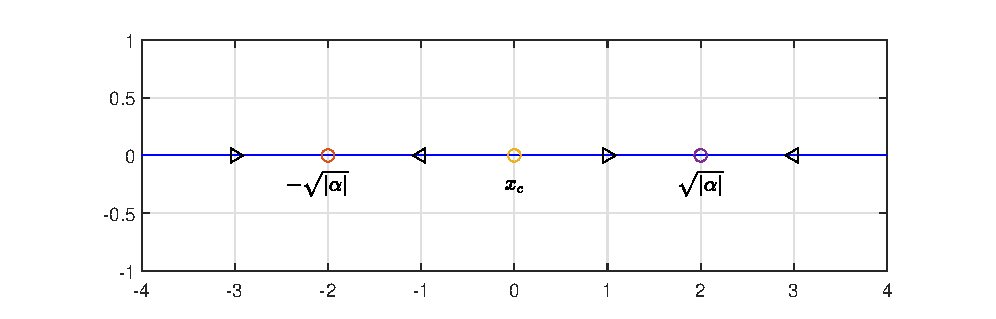
\includegraphics[width = 16cm, height = 5cm]{PhaseLine3a.eps}
			\end{figure}
			\newpage
			\item For $\alpha = 0$, we get one fixed point $x_c = 0$:
			\\ \\
			We can see that because $f'(0) = 0$, the critical point is half-stable. \\
			We can see that for $x < 0$, we get that $x' > 0$, and for $x > 0$, we get that $x' < 0$, thus giving us a sink.
			\begin{figure}[h!]
				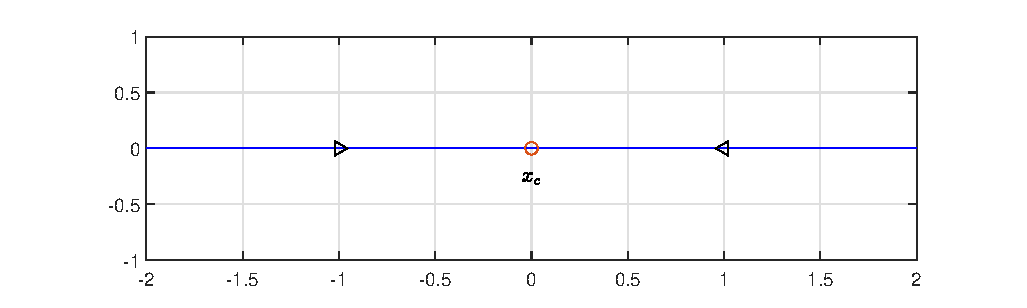
\includegraphics[width = 16cm, height = 5cm]{PhaseLine3b.eps}
			\end{figure}
			\item For $\alpha > 0$, we get one fixed point $x_c = 0$, we ignore the fixed point $x_c = i\sqrt{\alpha}$ because it is non-real:
			\\ \\
			We can see that because $f'(0) = -\alpha < 0$, the critical point is stable. \\
			We can see that for $x < 0$, we get that $x' > 0$, and for $x > 0$, we get that $x' < 0$, thus giving us a sink.
			\begin{figure}[h!]
				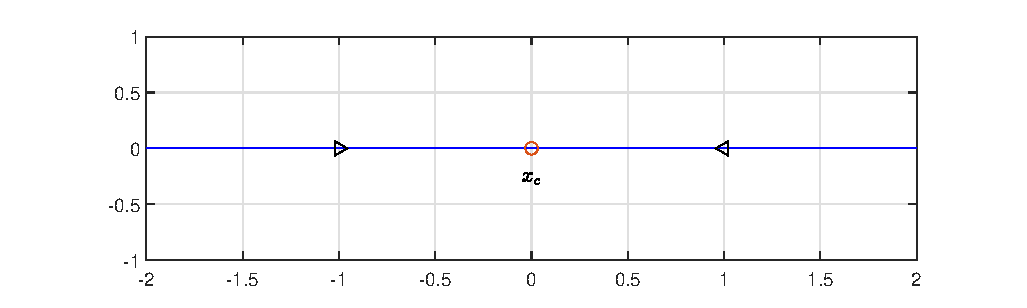
\includegraphics[width = 16cm, height = 5cm]{PhaseLine3b.eps}
			\end{figure}
			\item Notice that at $x_c = 0$, the fixed point changed from source to a sink as $\alpha$ changed. For $\alpha < 0$, $x_c = 0$ was a source, and for $\alpha \geq 0$, $x_c = 0$ was a sink. Also notice that $\forall x_c \in \{-\sqrt{|\alpha|},0,\sqrt{|\alpha|}\}, f'(x_c) = C\alpha$ with $C$ representing some constant.  Thus we have a bifurcation at $\alpha = 0$
		\end{enumerate}
		\newpage
		Let $\alpha \not= 0$, and let $x = \sqrt{r}$ with $\frac{dx}{dt} = \frac{1}{2 \sqrt{r}}\frac{dr}{dt}$. (Note that $x \not = -\sqrt{r}$, because we have that $x \geq 0$)
		\begin{align*}
			\frac{dx}{dt} &= -(\alpha x + x^3) & \frac{dr}{dt} &= -2r(\alpha + r ) \\
			\frac{1}{2 \sqrt{r}}\frac{dr}{dt} &= -\sqrt{r}(\alpha + r) & \frac{dr}{dt} + 2\alpha r&= -2r^2
		\end{align*}
		Now we can solve using Bernoulli's with $\mu = \frac{1}{r}$ and $\frac{d\mu}{dt} = \frac{-1}{r^2}\frac{dr}{dt}$
		\begin{align*}
			\frac{d\mu}{dt} - 2\alpha \mu &= 2 & \mu &= \frac{Ce^{2\alpha t} - 1}{\alpha}\\
			\int \frac{d\mu}{1 + \alpha\mu} &= \int 2\,dt & r &= \frac{\alpha}{Ce^{2\alpha t} - 1}
		\end{align*}
		Now we resubstitute $r = x^2$ and solve for C:
		\begin{align*}
			x &= \sqrt{\frac{\alpha}{Ce^{2\alpha t} - 1}} & C &= \frac{\alpha + x_0^2}{x_0^2} \\
			x(0) = x_0 &= \sqrt{\frac{\alpha}{C - 1}} & &= \frac{\alpha}{x_0^2} + 1\\
		\end{align*}
		Thus, we get the following:
			$$x = \sqrt{\frac{\alpha x_0^2}{(\alpha + x_0^2) e^{2\alpha t} - x_0^2}}$$
		\\
		For $\alpha < 0$, we can see that as $t \rightarrow -\infty$, $x \rightarrow 0$, and as $t \rightarrow \infty$, $x \rightarrow \sqrt{|\alpha|}$. 
		\\ \\ 
		For $\alpha > 0$, we can see that as $t \rightarrow -\infty$, we get undefined values of $x$, and as $t \rightarrow \infty$, $x \rightarrow 0$. 
		\\ \\ 
		\newpage 
		Let $\alpha = 0$, we get the following equation to solve:
		\begin{align*}
			\frac{dx}{dt} &= -x^3 & \frac{1}{-2x^2} &= -t + C \\
			\int \frac{dx}{x^3} &= \int -\,dt & x &= \sqrt{\frac{1}{2t + C}}
		\end{align*}
		If we let $x(0) = x_0$, we get the following solution:
		$$x = \sqrt{\frac{x_0^2}{2tx_0^2 + 1} }$$
		For $\alpha = 0$, we can see that as $t \rightarrow -\infty$, we get undefined values of $x$, and as $t \rightarrow \infty$, $x \rightarrow 0$.
	\end{problem}
	
	\begin{problem}{4}
		Analyze the following ODE with $\beta > 0$:
		$$\frac{dx}{dt} = \beta x(1 - x) - h$$
		for all values of the parameter $h > 0$
		\\ \\
		Let the following be true:
			$$f(x) = \beta x(1 - x) - h = -\beta x^2 + \beta x - h$$
		Notice we get the derivative $f'(x)$ as the following:
			$$f'(x) = -2\beta x + \beta$$
		We can find the fixed points $x_c$ using the quadratic formula:
		\begin{align*}
			x_c &= \frac{-\beta \pm \sqrt{\beta^2 - 4\beta h}}{-2\beta}
		\end{align*}
		Notice the following:
		\begin{align*}
			f'\left(\frac{-\beta + \sqrt{\beta^2 - 4\beta h}}{-2\beta}\right) = \sqrt{\beta^2 - 4\beta h} > 0 \\
			f'\left(\frac{-\beta - \sqrt{\beta^2 - 4\beta h}}{-2\beta}\right) = -\sqrt{\beta^2 - 4\beta h} < 0
		\end{align*}
		So we get that for all values, $\beta > 4h$, we get an unstable fixed point at $x_c = \frac{-\beta + \sqrt{\beta^2 - 4\beta h}}{-2\beta}$, and a stable fixed point at $x_c = \frac{-\beta - \sqrt{\beta^2 - 4\beta h}}{-2\beta}$
		\\ \\
		For values $\beta = 4h$, we get that the two earlier fixed points are the same, and get a half-stable fixed point, $x_c = \frac{1}{2}$ 
		\\ \\
		Lastly, for values $\beta < 4h$, we get no real fixed points.
	\end{problem}

\end{document}
